\section{Introduction}

% \setLayout{mainpoint}

\begin{frame}[noframenumbering, plain]{}
    \frametitle{Introduction}
\end{frame}

% \setLayout{vertical}

%---------------------------------------------------------
\begin{frame}
    \frametitle{Cell Cultures}
    \begin{columns}
        \column{0.5\textwidth}
            \begin{itemize}
                \item<1-> Vital to applications in:
                \begin{itemize}
                    \item<2-> Industry.
                    \item<3-> Academics.
                \end{itemize}
            \end{itemize}
            
                \begin{figure}[!htb]
                    \centering
                    \visible<6->{\subfloat{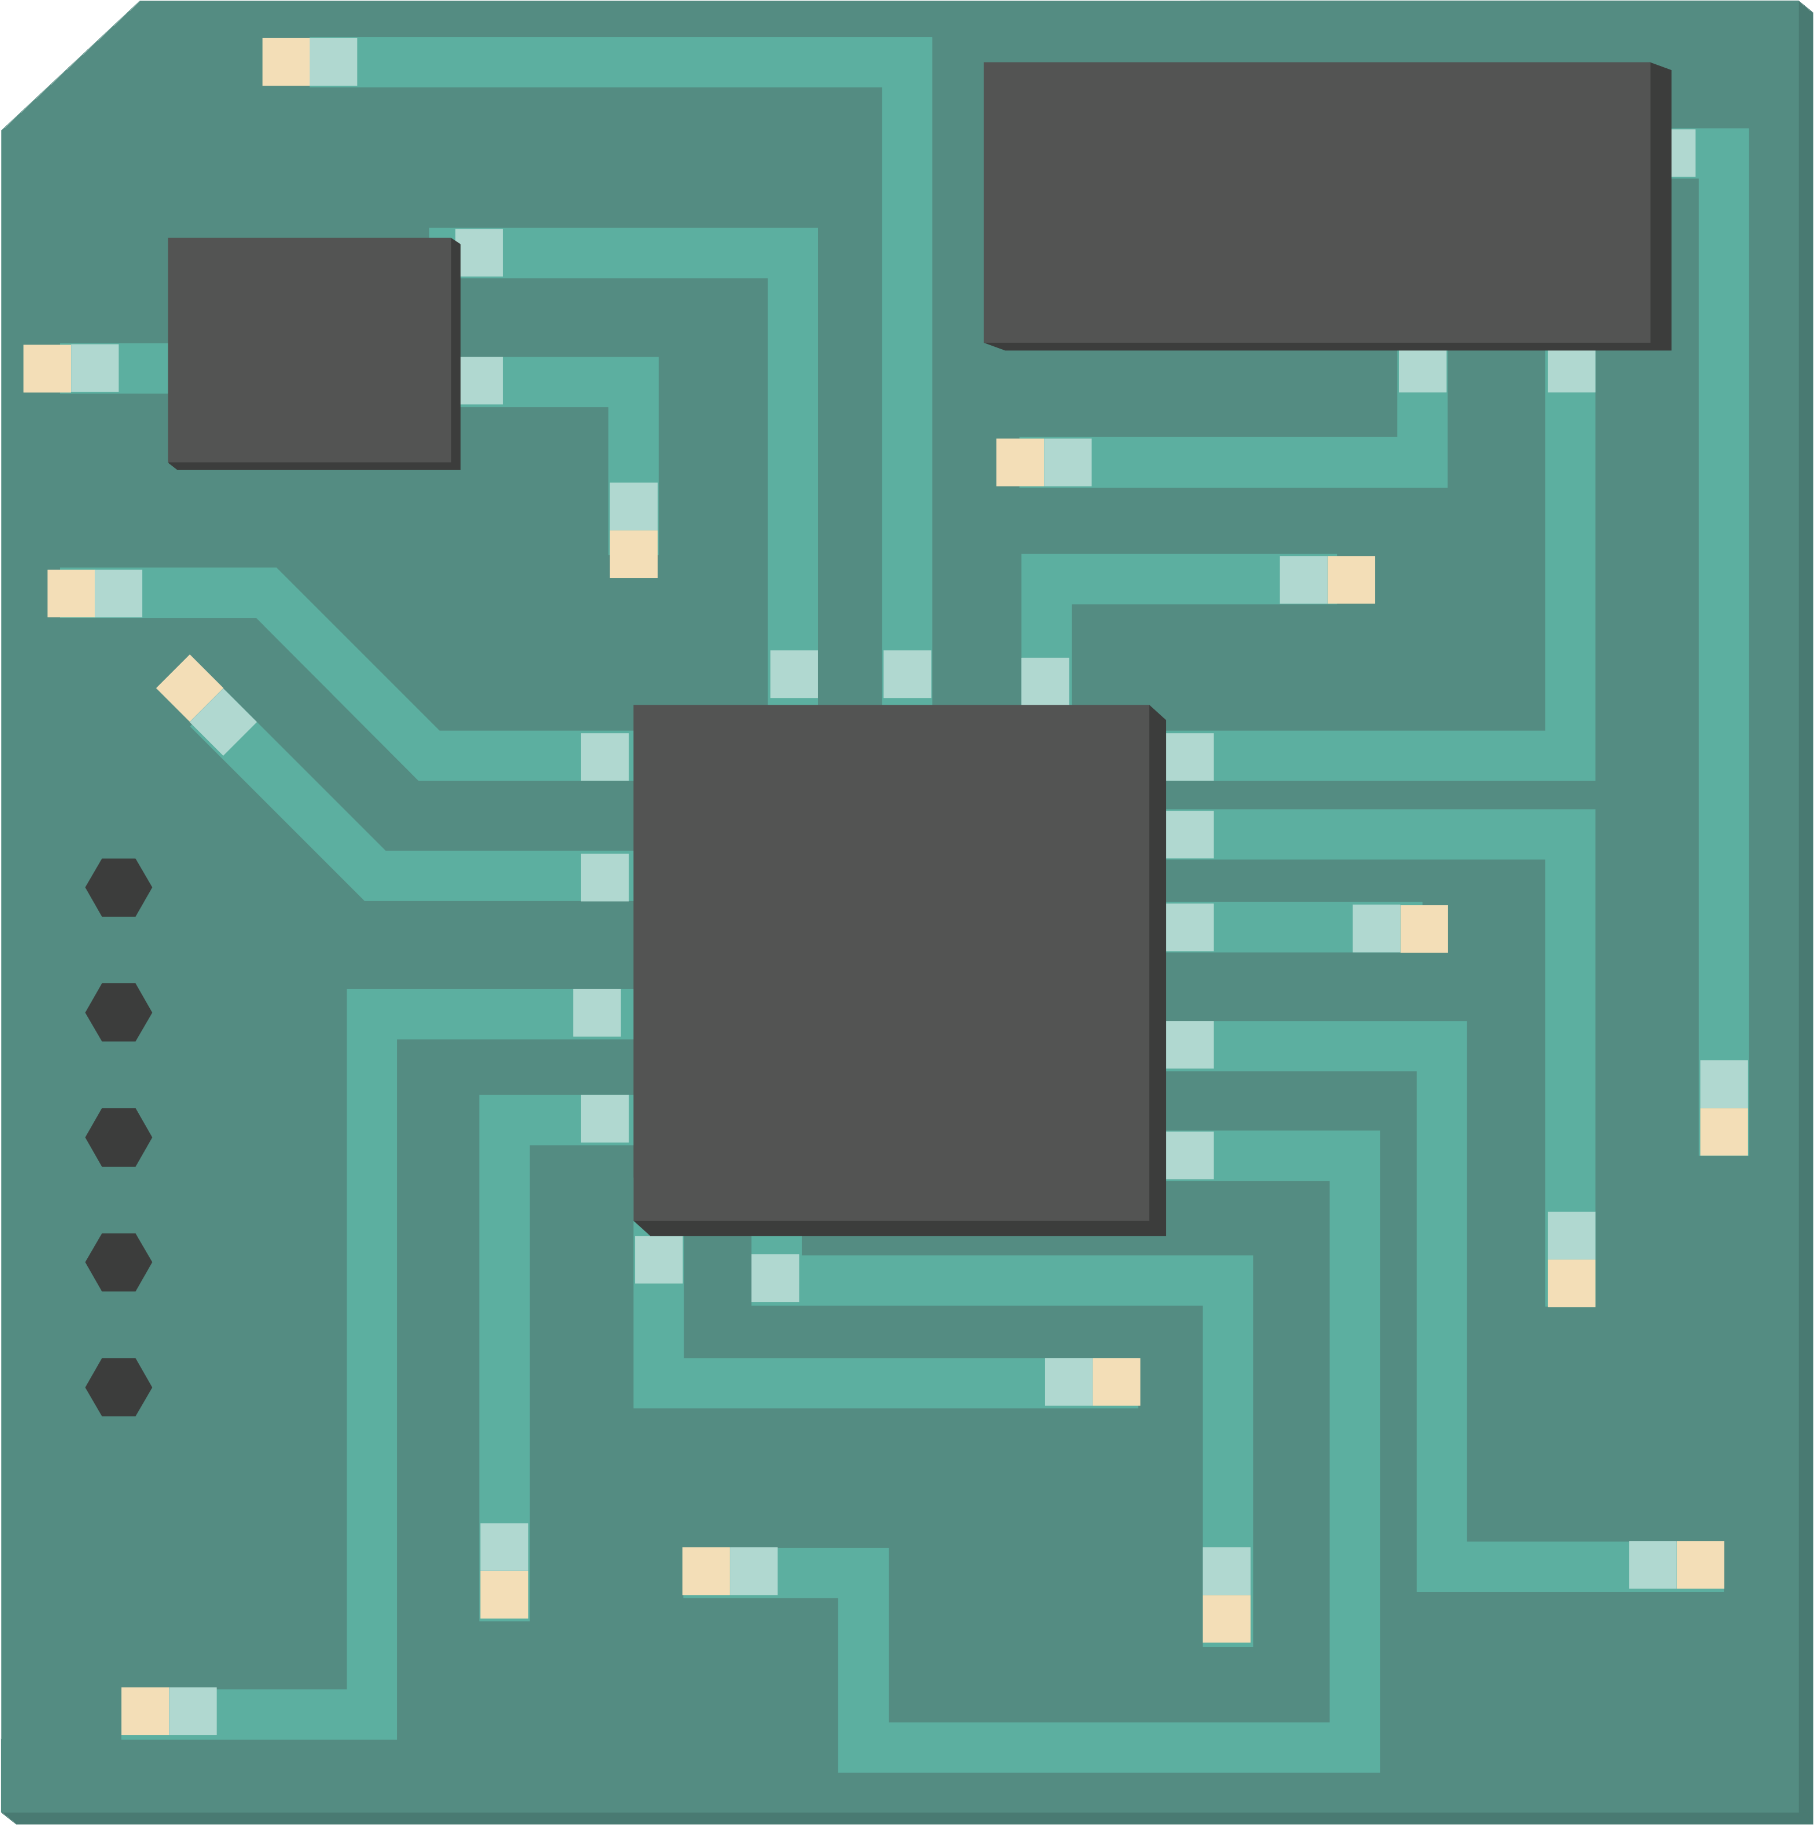
\includegraphics[width=1.5cm]{figures/introduction/in_silico}} \hspace*{0.3cm}
                    \subfloat{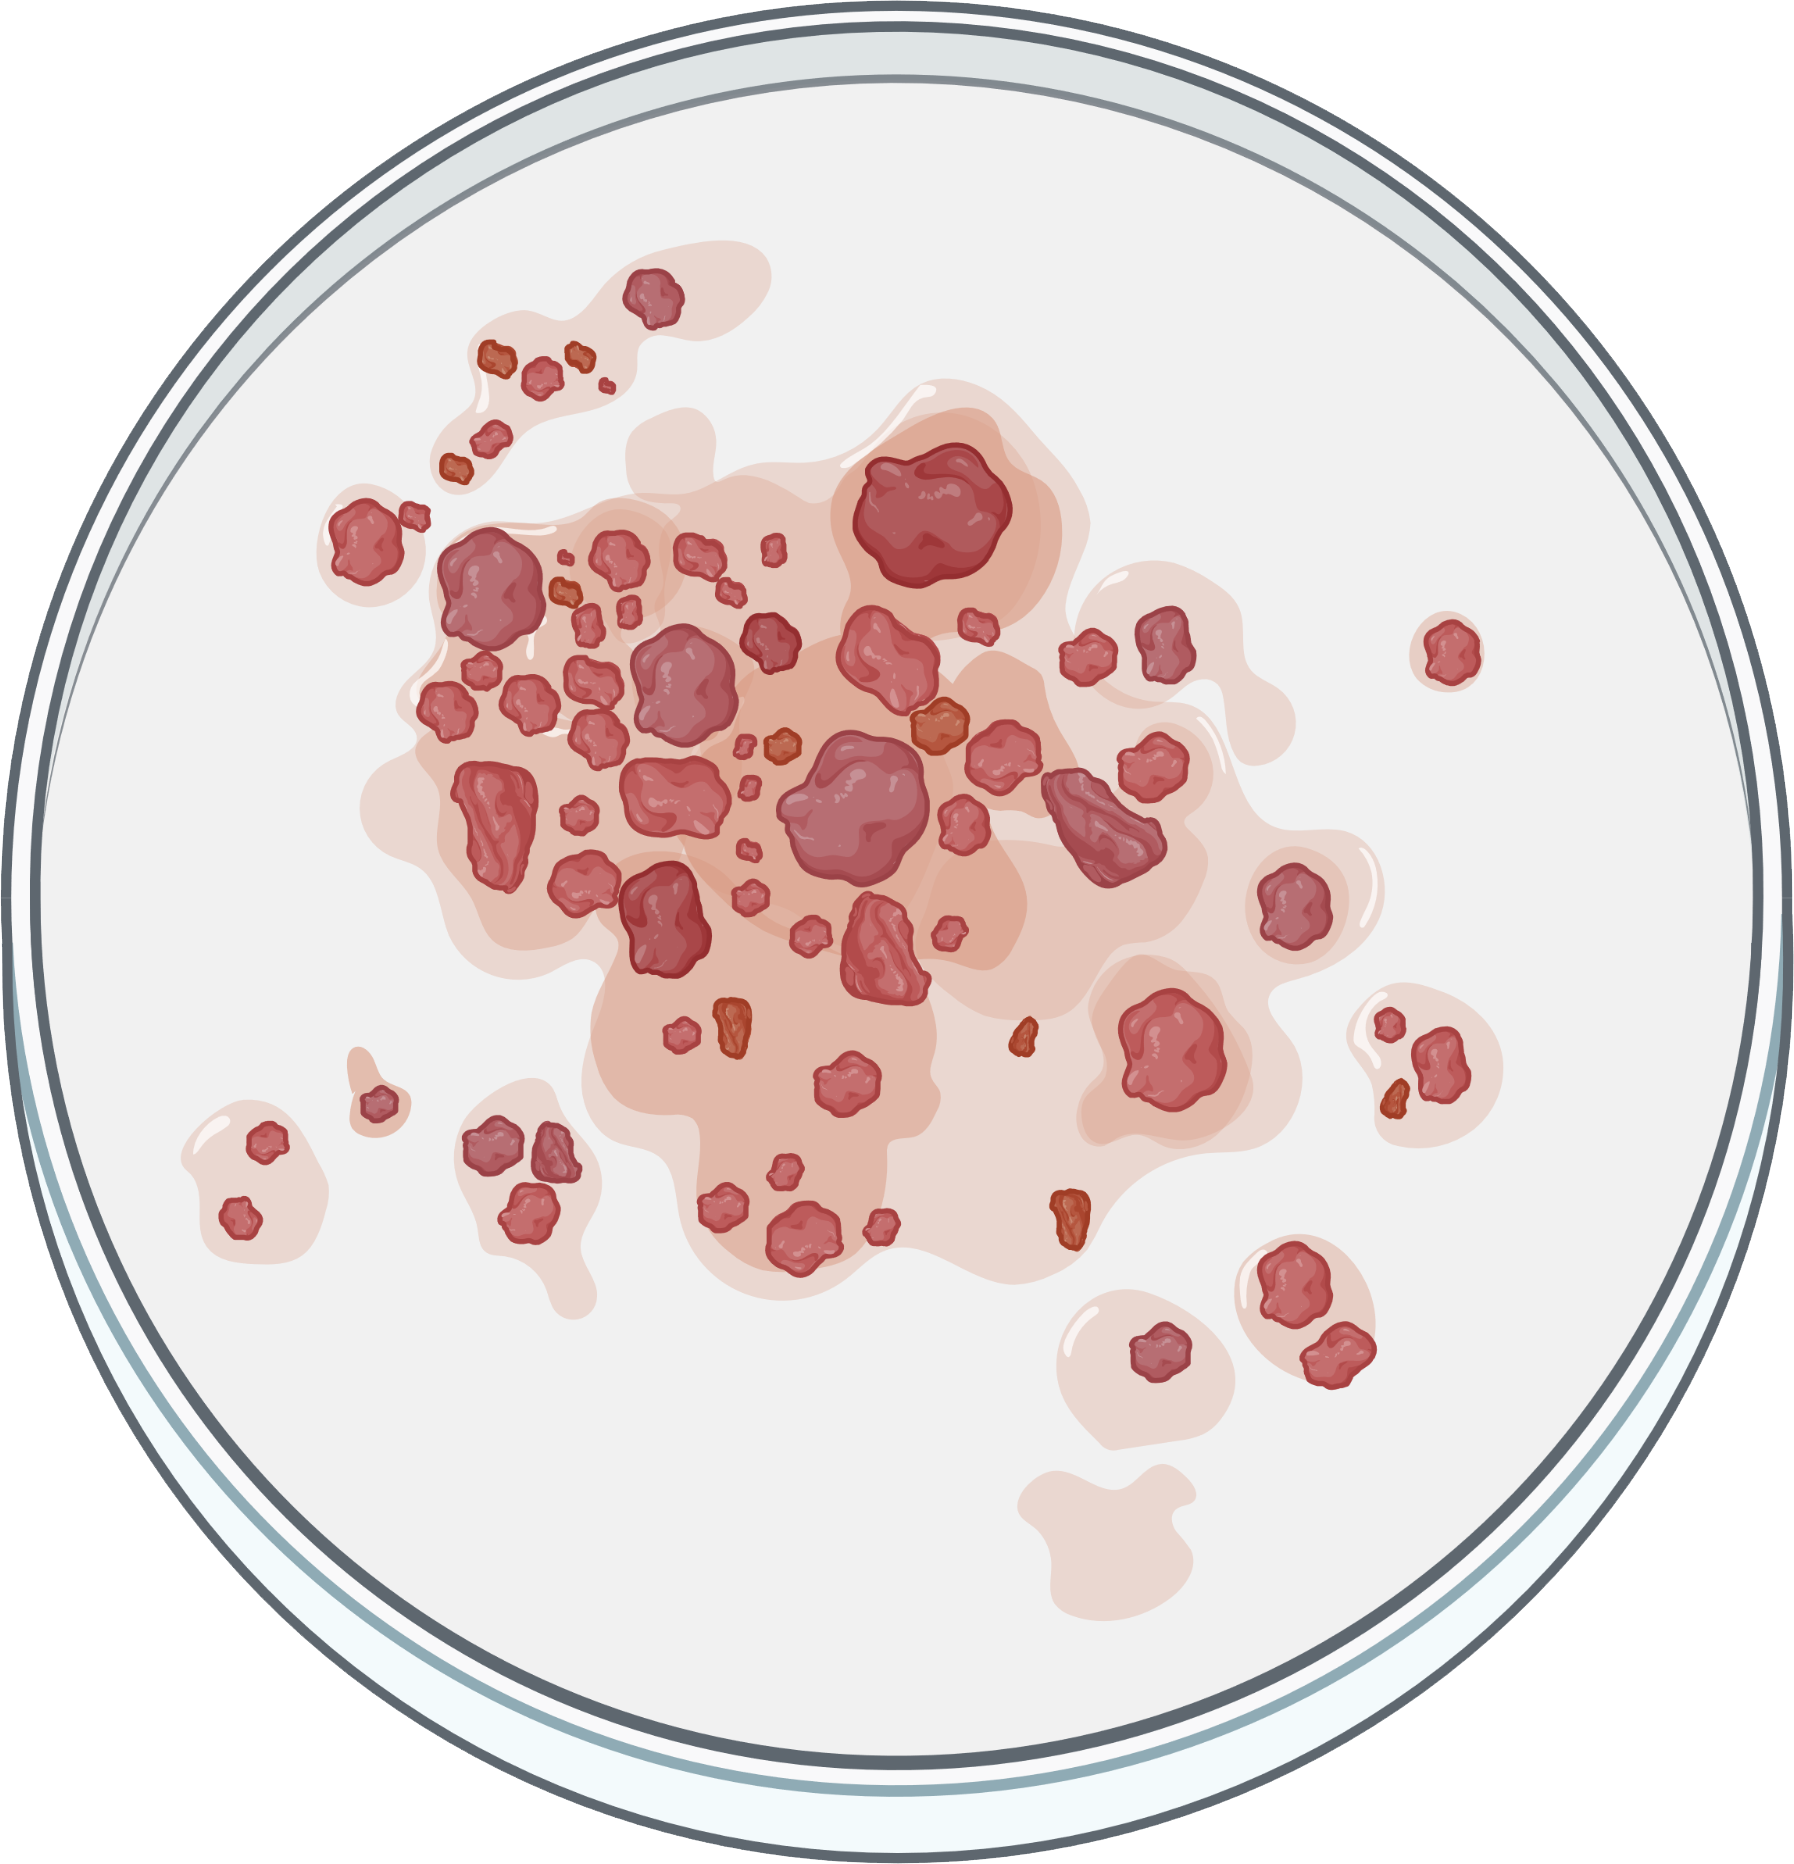
\includegraphics[width=1.5cm]{figures/introduction/in_vitro}} \hspace*{0.3cm}
                    \subfloat{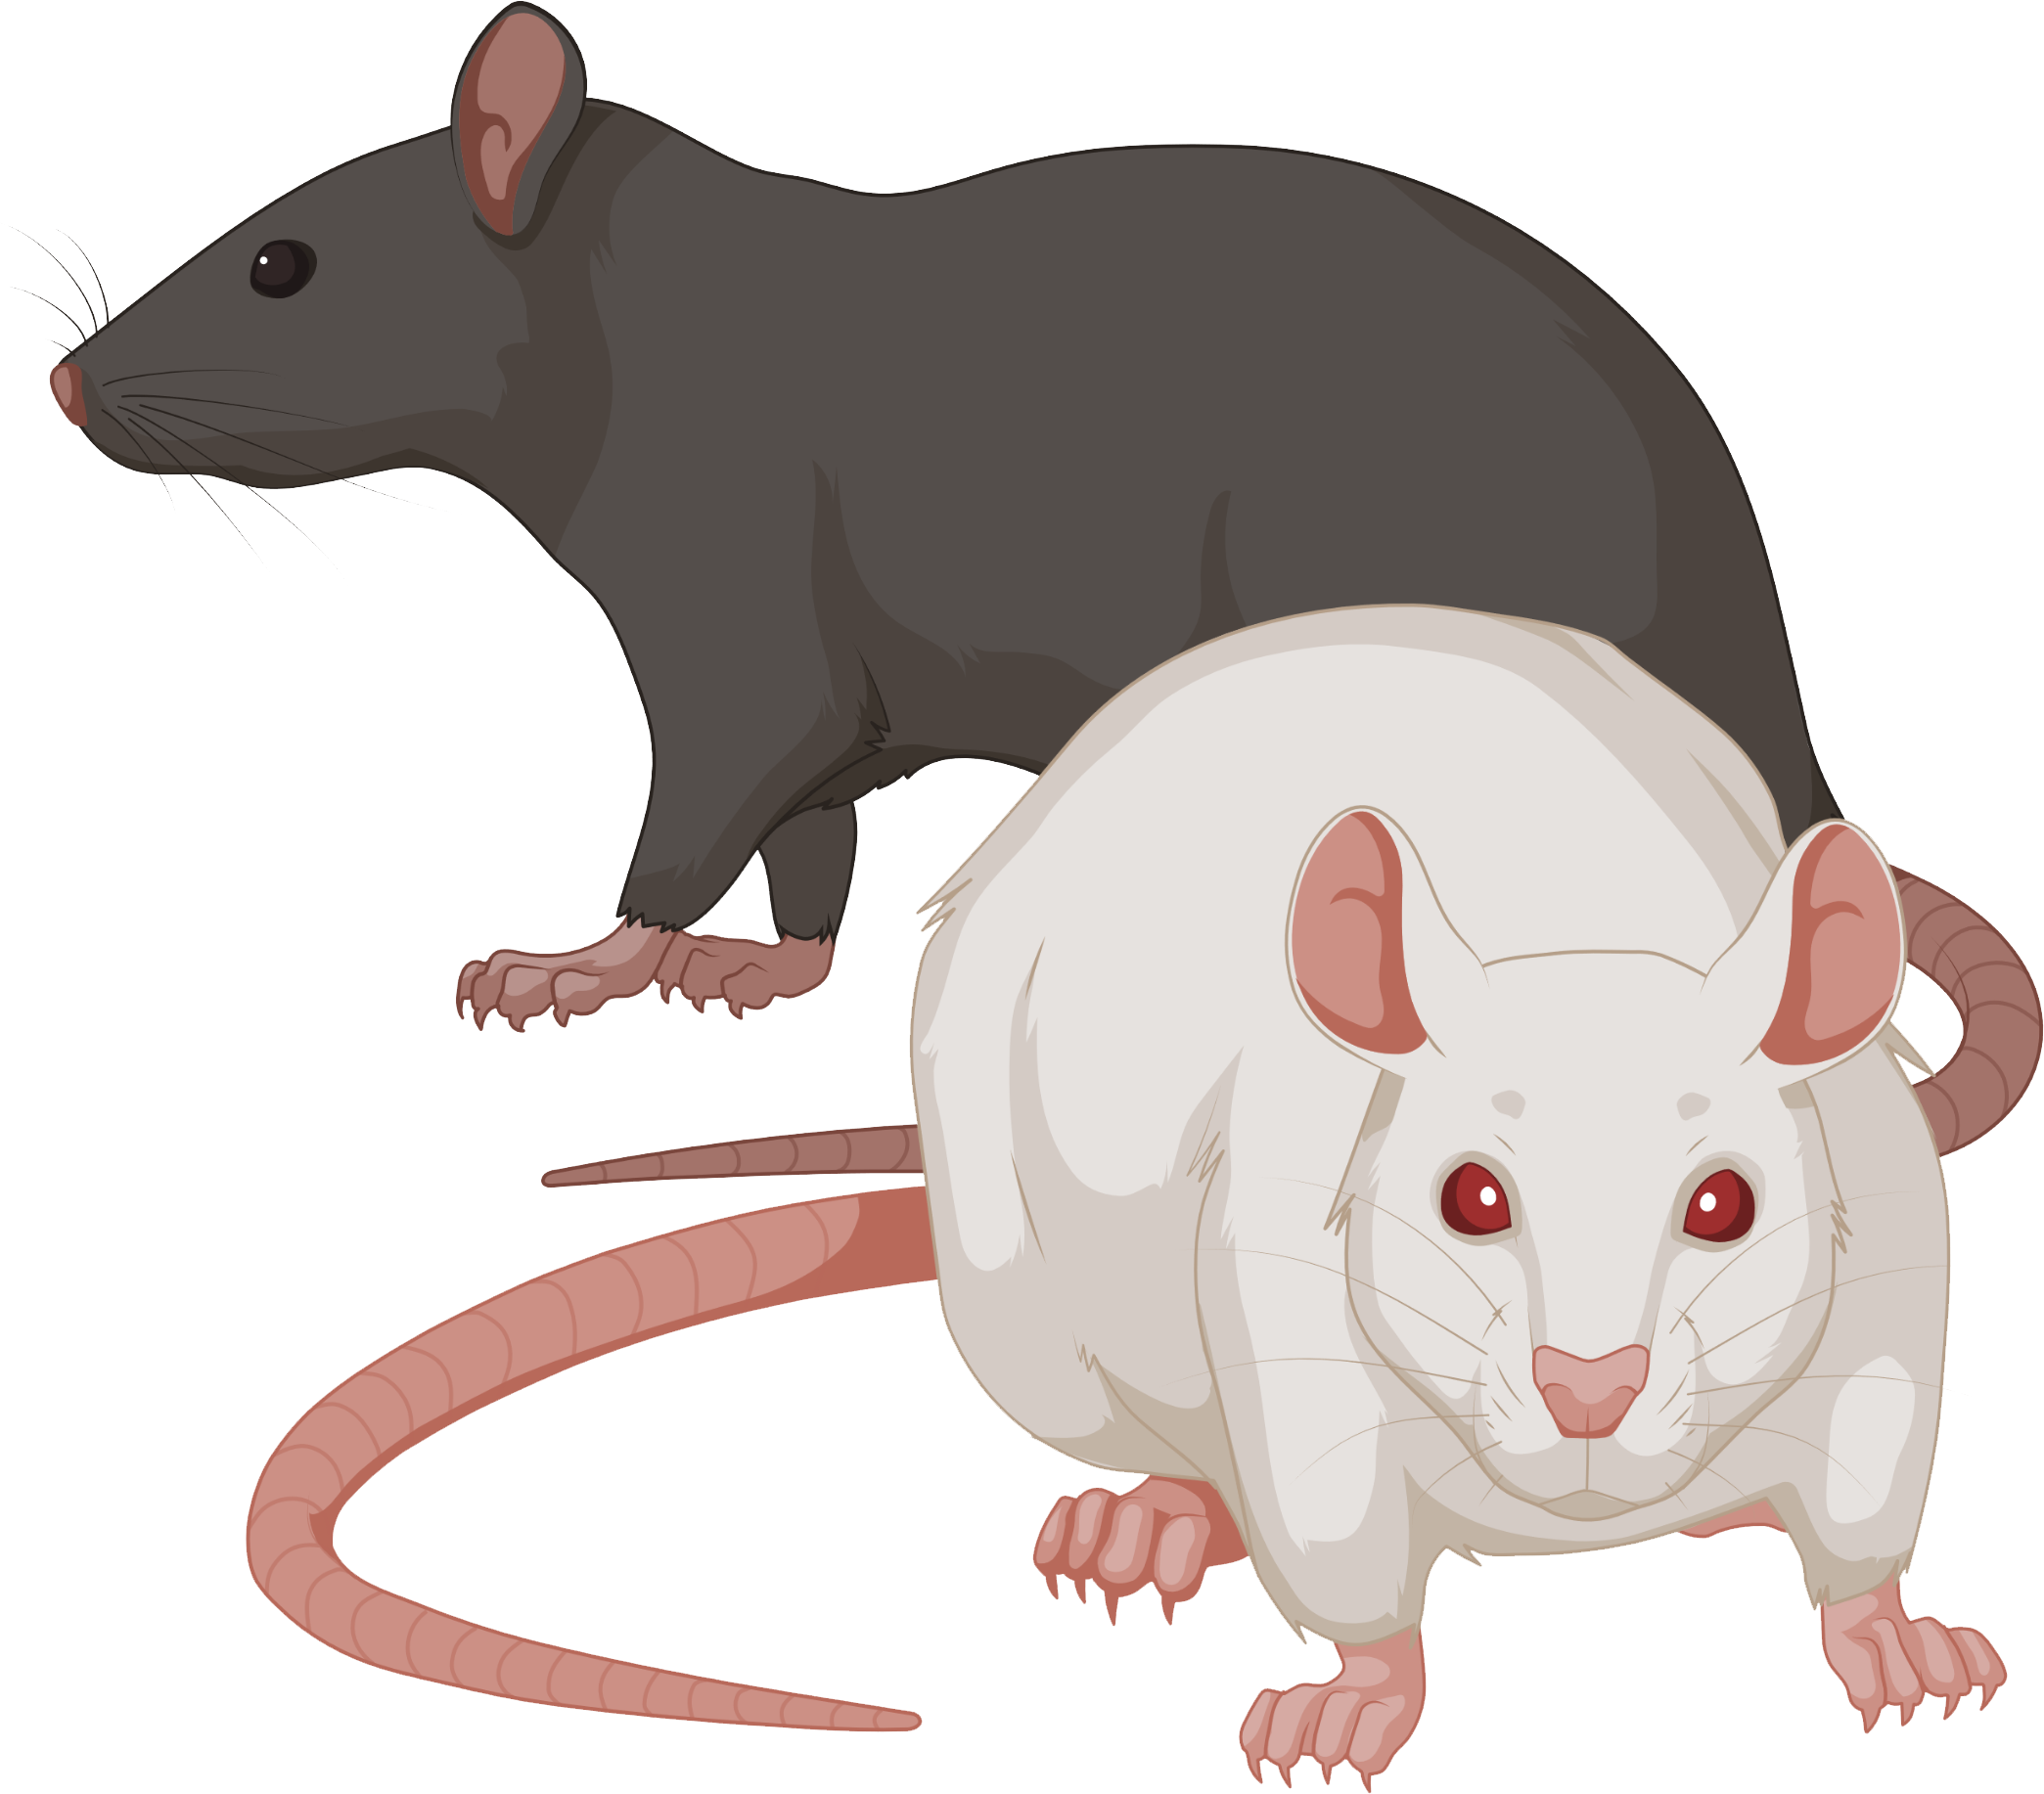
\includegraphics[width=1.5cm]{figures/introduction/in_vivo}}\\
                    Pre-Clinical}
                    \visible<7->{\subfloat{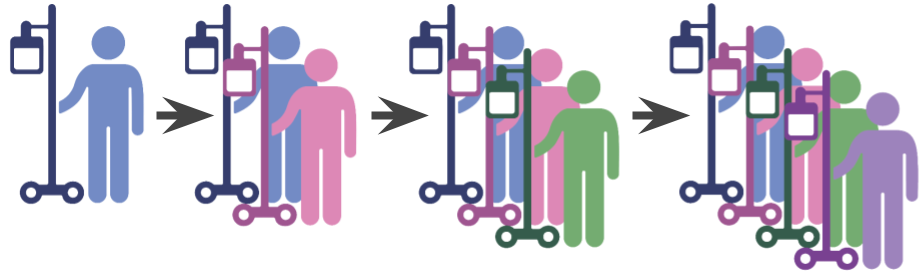
\includegraphics[width=5cm]{figures/introduction/clinical}}\\
                    Clinical}
                \end{figure}
        \column{0.5\textwidth}
            \begin{itemize}    
                \item<4-> Pharmaceutical context:
                    \begin{itemize}
                        \item<5-> Drug discovery and development.
                        \begin{itemize}
                            \item<6-> Pre-Clinical.
                            \item<7-> Clinical trials.
                        \end{itemize}
                    \end{itemize}
            \end{itemize}
    \end{columns}
\end{frame}

%---------------------------------------------------------
\begin{frame}{Drug Discovery}
    \begin{figure}[!htb]
    \centering
    \setbeamercovered{transparent}
    \visible<1->{\subfloat[\textit{in silico}]{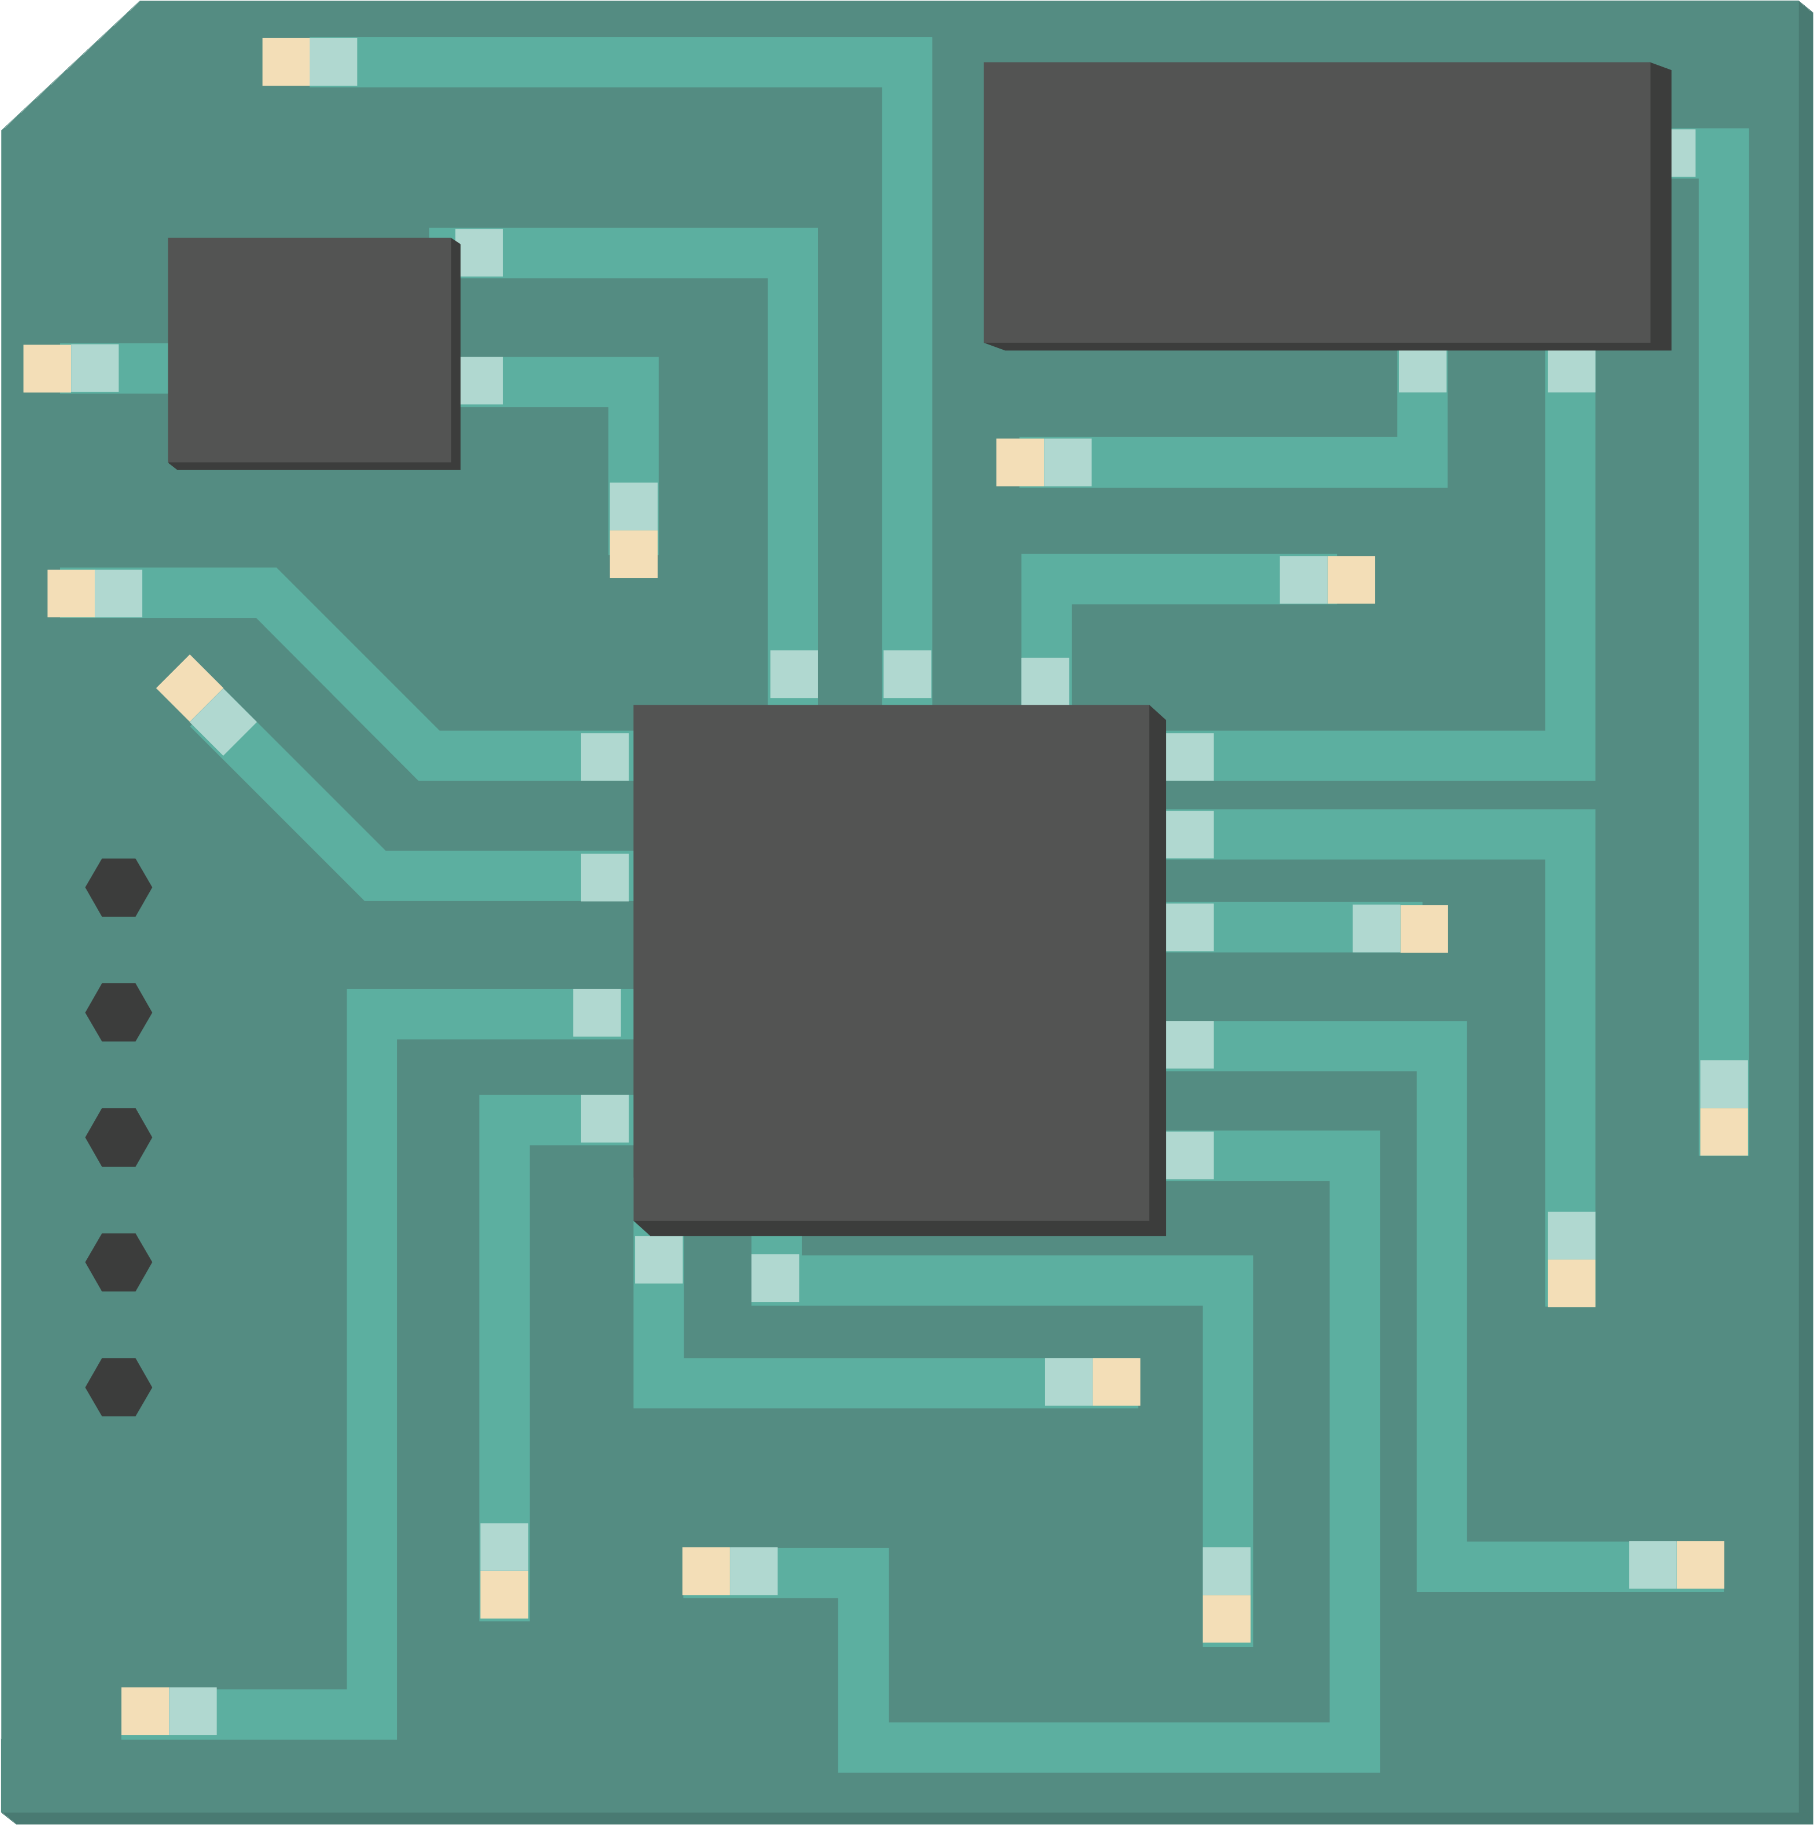
\includegraphics[width=2cm]{figures/introduction/in_silico}} \hspace*{0.3cm}}
    \visible<2->{\subfloat[\textit{in vitro}]{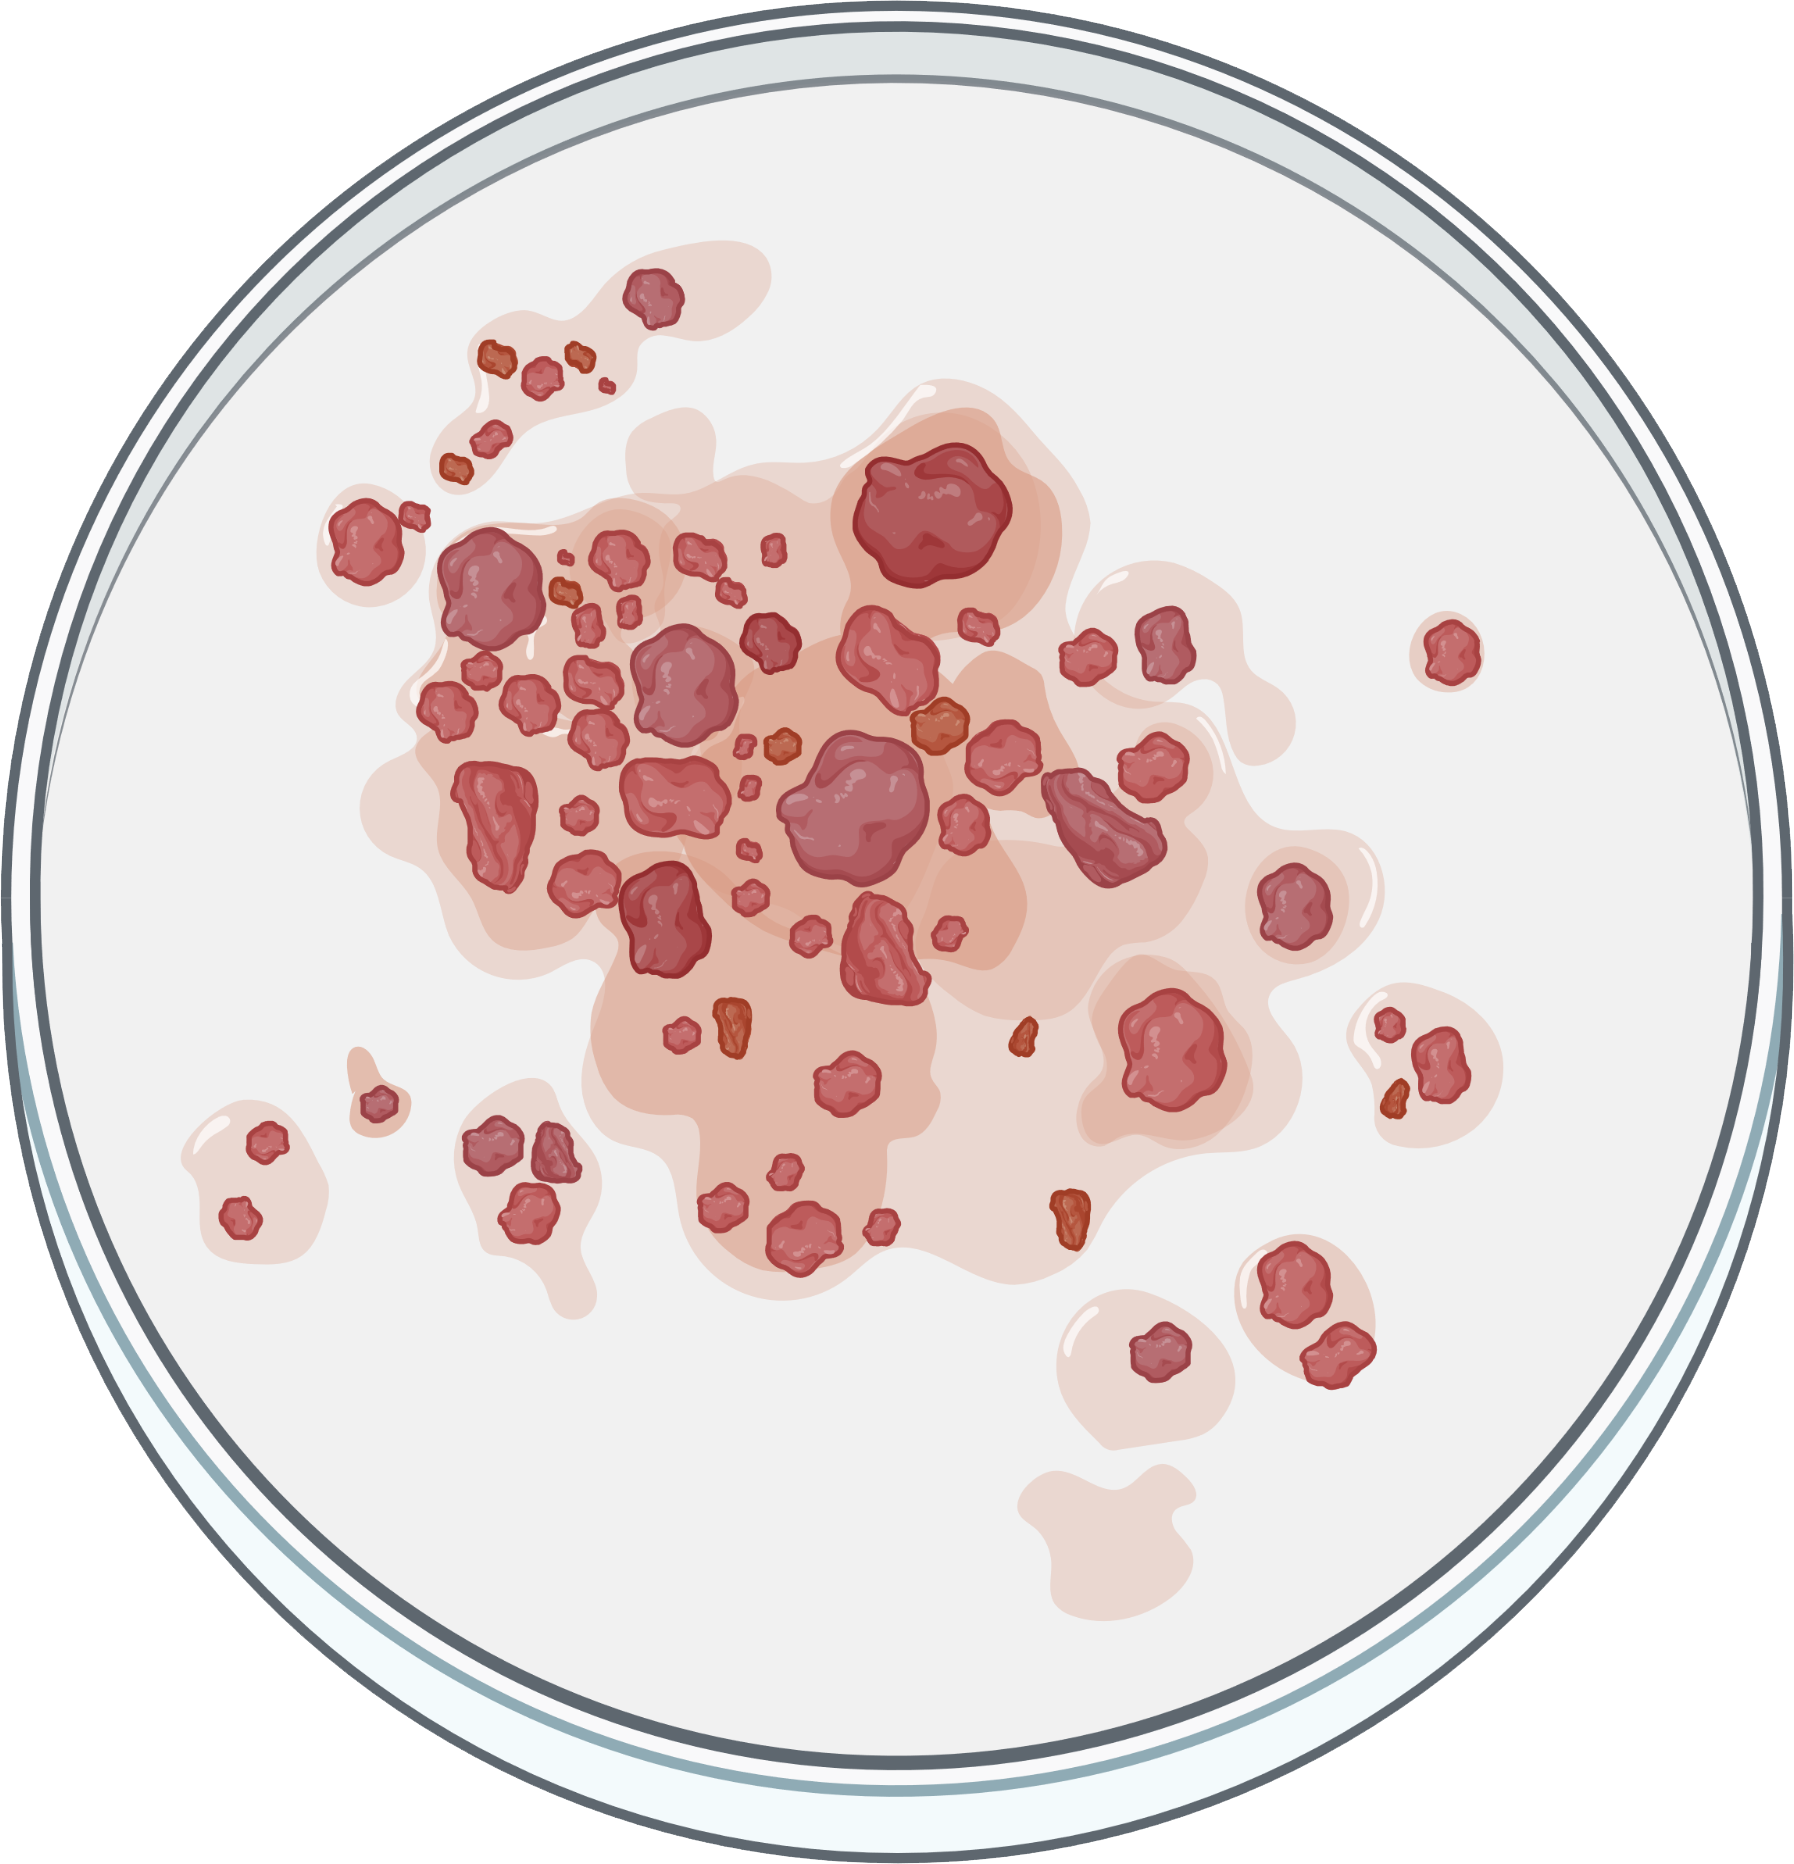
\includegraphics[width=2cm]{figures/introduction/in_vitro}} \hspace*{0.3cm}}
    \visible<3->{\subfloat[\textit{in vivo}]{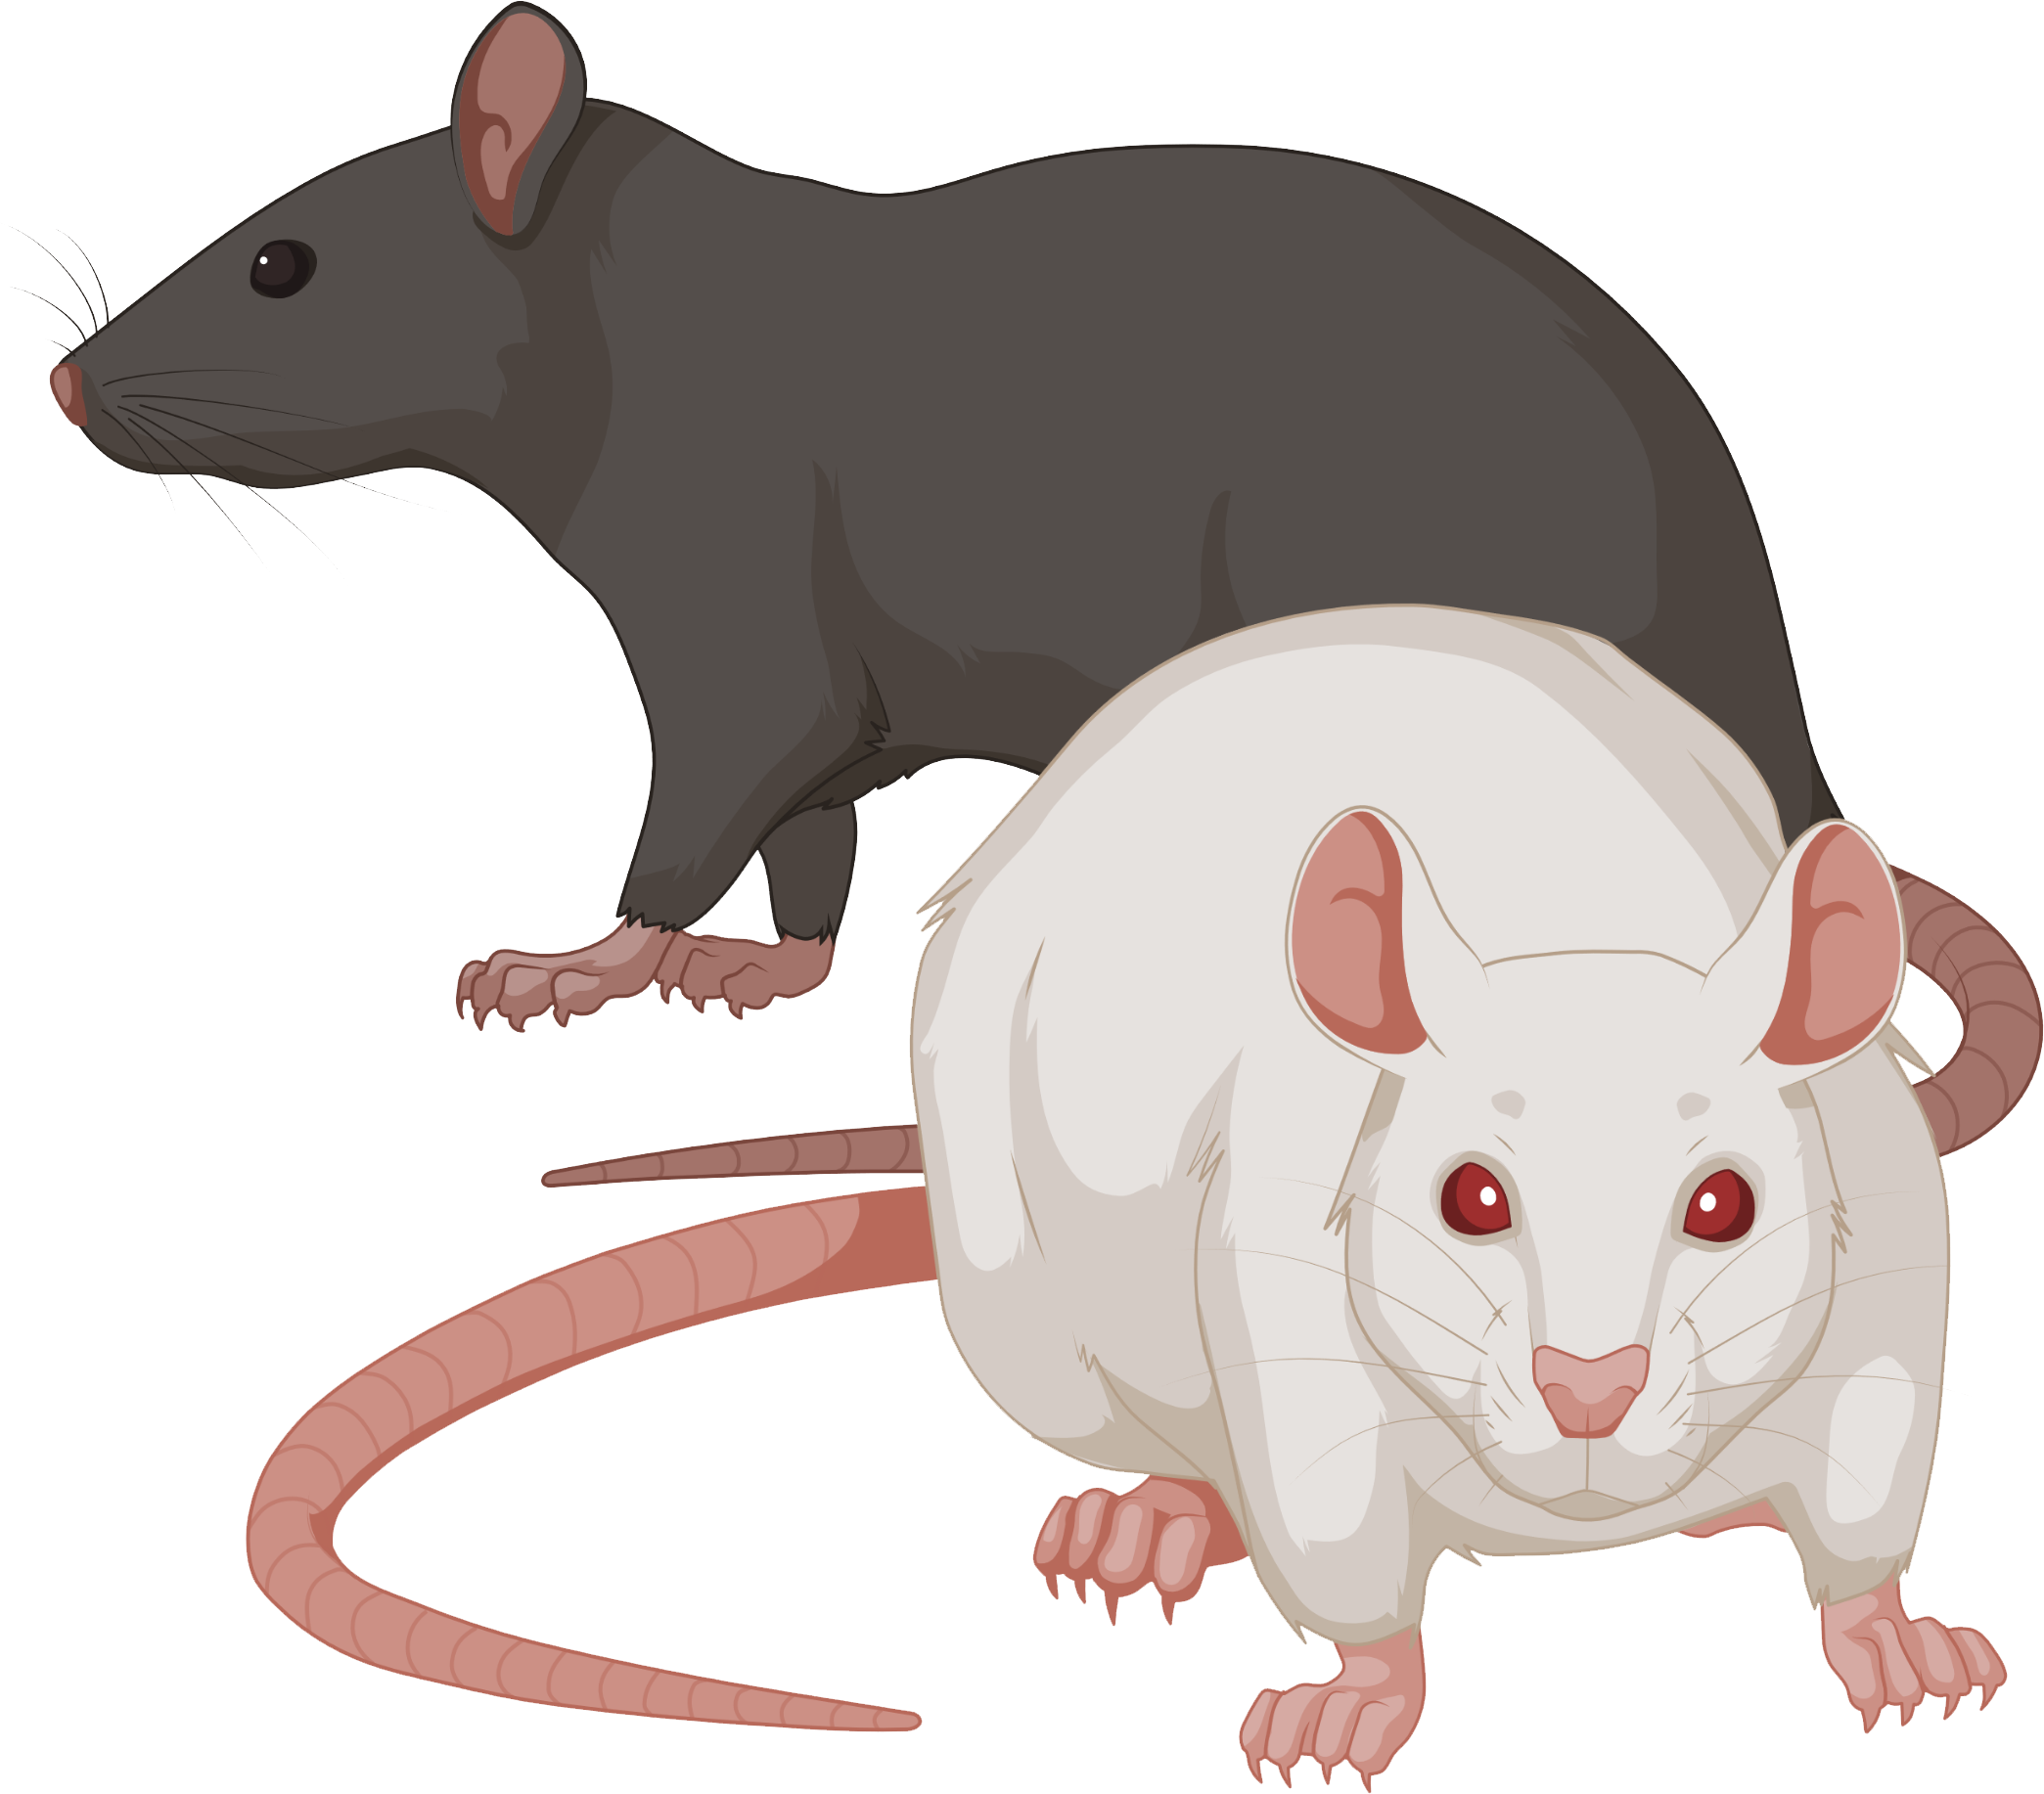
\includegraphics[width=2cm]{figures/introduction/in_vivo}}}\\
    \visible<4->{\subfloat[Clinical Trials]{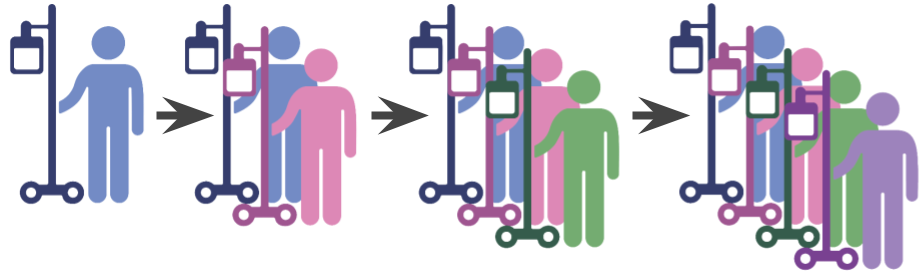
\includegraphics[width=9cm]{figures/introduction/clinical}}}
    \end{figure}
\end{frame}

%---------------------------------------------------------
\begin{frame}{Drug Discovery}
    \begin{columns}
        \column{0.4\textwidth}
            \begin{itemize}
                \item<1-> This process is:
                \begin{itemize}
                    \item<2-> Laborious.
                    \item<3-> Expensive.
                    \item<4-> Time consuming.
                \end{itemize}
                \item<5-> Low success rate:
                \begin{itemize}
                    \item<6-> Only \alert{10\%} moves to clinical trials.
                \end{itemize}
            \end{itemize}
        \column{0.4\textwidth}
            \begin{itemize}
                \item<7-> Fails are attributed to \alert{pre-clinical} stages.
                \begin{itemize}
                    \item<8-> Too simple.
                    \item<9-> Failed to eliminate bad candidates.
                \end{itemize}
            \end{itemize}
    \end{columns}
\end{frame}

%---------------------------------------------------------
\begin{frame}{2D Cultures}
    \begin{columns}
        \column{0.45\textwidth}
        \begin{itemize}
            \item<1-> Most common culture.
            \item<2-> Cells grow:
            \begin{itemize}
                \item<3-> In the culture medium.
                \item<4-> Monolayer.
                \item<5-> Attached to the substrate.
            \end{itemize}
        \end{itemize}

        \begin{figure}[!htb]
            \centering
            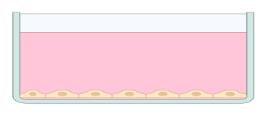
\includegraphics[width=6cm]{figures/introduction/2D_culture}
        \end{figure}

        \column{0.5\textwidth}
        \begin{itemize}
            \item<6-> Practical to evaluate compounds, since:
            \begin{itemize}
                \item<7-> No ethical committee required.
                \item<8-> Widespread training of personnel.
                \item<9-> Immortalized cells.
                \item<10-> Cells are genetically similar.
                \item<11-> Cells can be frozen.
                \item<12-> Cheaper upkeep.
            \end{itemize}
            \item<13-> Downside:
                \begin{itemize}
                    \item<14-> Can't reproduce microenvironment.
                \end{itemize}
        \end{itemize}
    \end{columns}
\end{frame}

%---------------------------------------------------------
\begin{frame}{3D Cultures}
    \begin{columns}
        \column{0.45\textwidth}
        \begin{figure}[!htb]
            \centering
            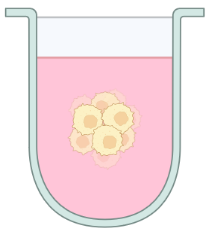
\includegraphics[width=6cm]{figures/introduction/3D_culture}
        \end{figure}

        \column{0.5\textwidth}
        \begin{itemize}
            \item<1-> Cells grow:
                \begin{itemize}
                    \item<1-> Floating in the culture medium.
                    \item<2-> With or without scaffolding.
                \end{itemize}
            \item<3-> Microenvironment reproduction:
            \begin{itemize}
                \item<4-> Cell-to-cell communication.
                \item<5-> Interactions between stroma and cell.
                \item<6-> Cell differentiation.
            \end{itemize}
            \item<7-> Better \textit{in vitro} alternative:
            \begin{itemize}
                \item<8-> Faster testing.
                \item<9-> Automation.
                \item<10-> Reproducibility.
            \end{itemize}
        \end{itemize}
    \end{columns}
\end{frame}

%---------------------------------------------------------
\begin{frame}{Spheroid Regions}
    \begin{figure}
        \centering
        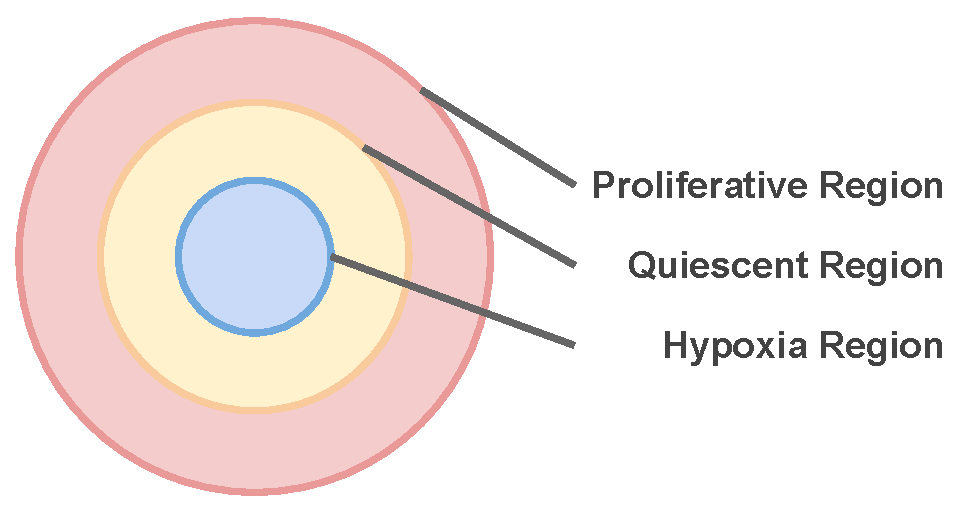
\includegraphics[width=8cm]{figures/introduction/spheroid_regions}
        \label{fig:spheroid_regions}
    \end{figure}
\end{frame}

%---------------------------------------------------------
\begin{frame}{Research Questions}
        \begin{enumerate}
            \item Shape-aware \alert{loss function affects} segmentation?
            \item Is the U-net encoder a \alert{better generator backbone} for spheroid segmentation?
            \item Can we evaluate spheroids with \alert{destroyed proliferative zones}?
            \item Is \alert{scale} important in spheroid segmentation?
            \item Can a single GAN \alert{differentiate all three spheroid zones}?
        \end{enumerate}
\end{frame}

%---------------------------------------------------------
% \setLayout{horizontal}

\begin{frame}{Objectives}
            \begin{block}{Global Objectives}
                \begin{columns}
                \column{0.5\textwidth}
                \begin{enumerate}
                    \item Create the spheroid image\\ dataset (SDSS).
                \end{enumerate}
                \column{0.5\textwidth}
                \begin{enumerate}
                \setcounter{enumi}{1}
                    \item A self-supervised semantic segmentation method.
                \end{enumerate}
                \end{columns}
            \end{block}
            \begin{block}{Specific Objectives}
                \begin{columns}
                \column{0.5\textwidth}
                \begin{enumerate}
                    \item Literature review.
                    \item Setup dataset.
                    \item Select metric.
                    \item Develop method.
                    \item Evaluate Loss functions.
                \end{enumerate}
                \column{0.5\textwidth}
                \begin{enumerate}
                \setcounter{enumi}{5}
                    \item Select GAN backbones.
                    \item Process results.
                \end{enumerate}
                \end{columns}
            \end{block}
\end{frame}

%---------------------------------------------------------
% \setLayout{vertical}

\begin{frame}{Expected Challenges}
    \begin{itemize}
        \item Access to data.
        \item Lack of protocols.
        \item Heterogeneous evaluation metrics.
        \item GANs convergence.
        \item Annotate images.
        \item Train with few samples.
    \end{itemize}
\end{frame}

%---------------------------------------------------------
\begin{frame}{Expected Contributions}
    \begin{itemize}
        \item New public dataset.
        \item New self-supervised segmentation method.
        \item Segmentation as an analysis tool.
        \item Qualitative study.
        \item Competitive results.
    \end{itemize}
\end{frame}
